\section{Moto circolare uniformemente accelerato}
%-----------------------------------------------------------------------------
Il moto circolare non uniforme si ha quando la velocità angolare non è
costante nel tempo. Questo comporta che la componente tangente di $\vec a$ non è nulla. Nel caso in cui $\omega$ è lineare nel tempo si avrà un moto circolare uniformemente accelerato.
\\ Definiamo quindi l'accelerazione angolare:
\begin{equation}
    \alpha_{(t)} = \dot \omega = \ddot \phi\seg a_t = \dot v =
    \frac d{dt}\sx \omega R\dx = \alpha R
\end{equation}
Di conseguenza avremo che:
\begin{multline}
    \omega_{(t)} = \omega_0 + \int_{t_0}^tdt'\alpha_{(t')}  = \omega_0 + \alpha_0\sx t - t_0\dx \seg
    \\\boxed{\phi_{(t)} = \phi_0 + \omega_0\sx t - t_0\dx+ \frac12\alpha_0\sx t - t_0\dx^2}
\end{multline}
Esiste anche un analogo della formula (\ref{eq:v(x)_0}).
\begin{equation}
    \alpha =\dot \omega = \frac{d\omega}{d\phi}\dot\phi\seg
    \boxed{\omega^2_{(\phi)} = \omega_0^2 + 2\alpha_0\sx\phi-\phi_0\dx}
\label{eq:w(phi)}
\end{equation}
Osservando la figura (\ref{fig:rotantvector}), possiamo scrivere la relazione
tra velocità e velocità angolare con un formalismo verroriale:

\begin{figure}[htbp]
    \centering
        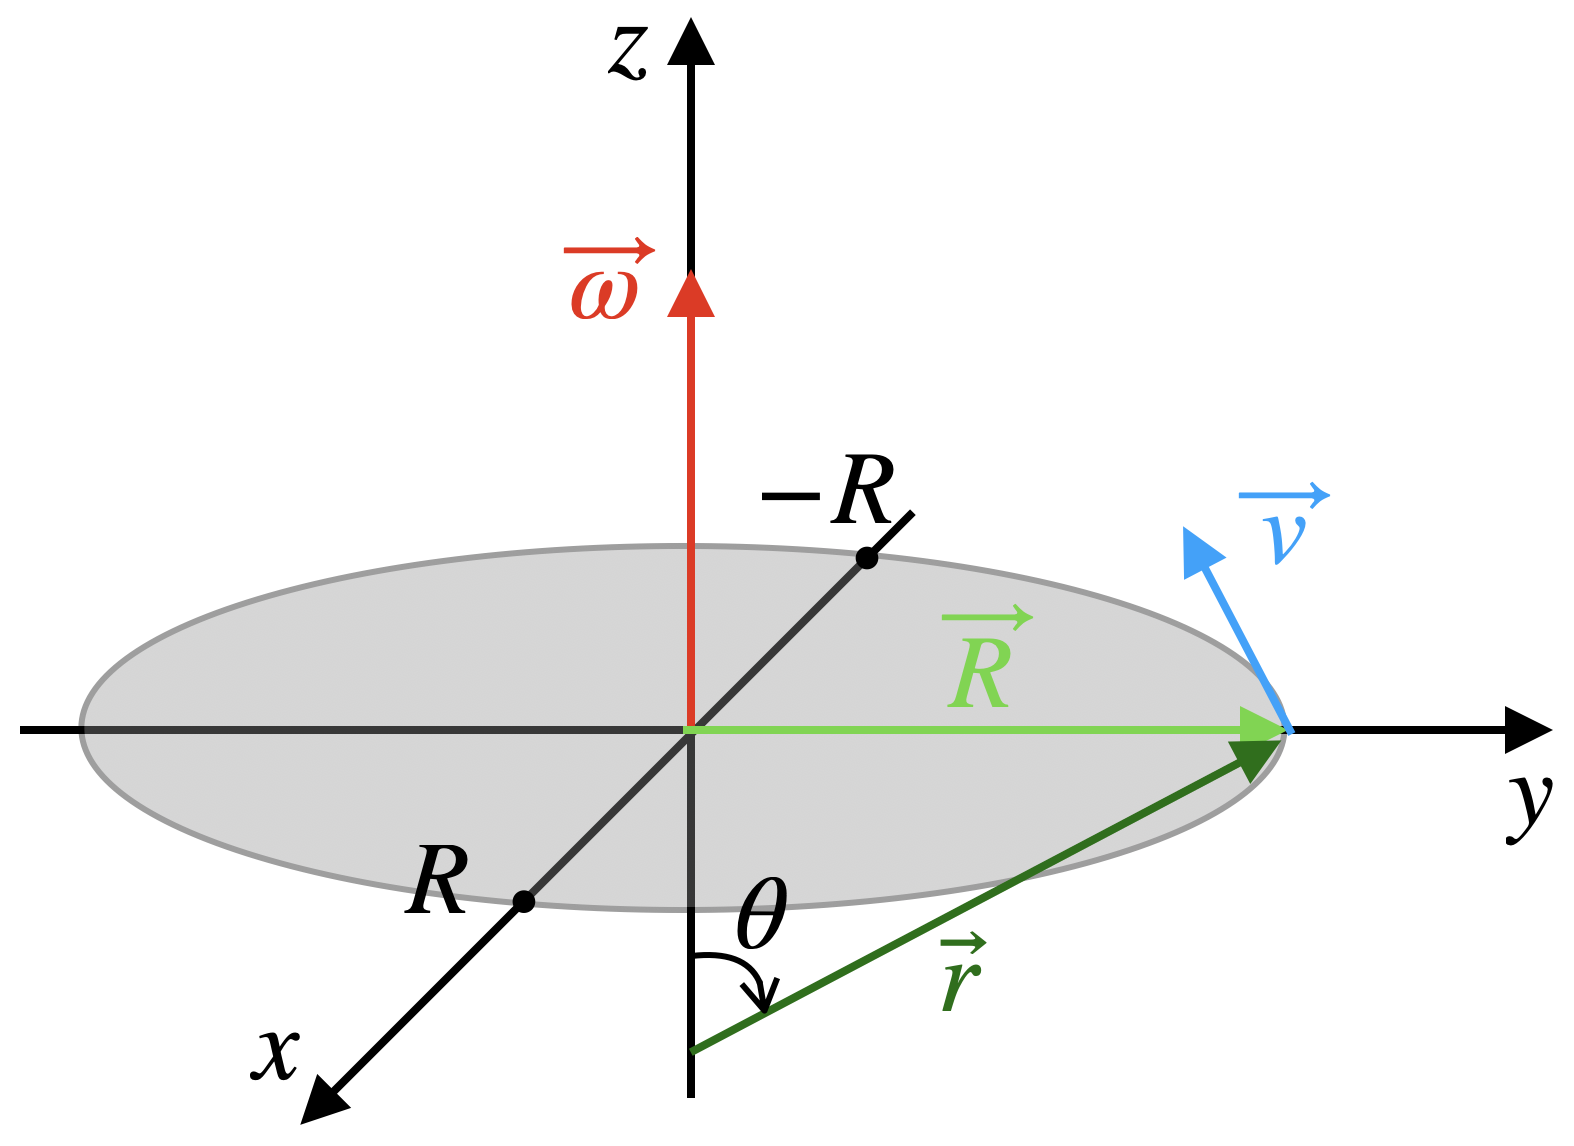
\includegraphics[width=7cm]{images/ovetr.png}
        \caption{Rappresentazione dei vettori $\vec\omega$ e $\vec v$ in un moto
        circolare per $\vec R$ e di precessione per $\vec r$.}
\label{fig:rotantvector}
\end{figure}

\begin{equation}
    \vec v = \vec\omega\times\vec R\seg \left| \vec v \right|  = \omega R
\end{equation}
Se trasliamo verso il basso l'origine degli assi otteniamo che:
\begin{equation}
    \vec v = \vec\omega\times\vec r\seg \left| \vec v \right|  = \omega r\sin\theta = \omega R
\label{eq:v(w)}
\end{equation}
Ne segue che dato un vettore generico rotante $\vec A$ avremo che:
\begin{equation}
    \frac{d\vec A}{dt} = \vec\omega\times\vec A
\label{eq:rotantvector}
\end{equation}
Infine scriviamo la forma dell'accelerazione.
\begin{equation}
    \vec a = \frac d{dt}\sx\vec\omega\times\vec r\dx =
    \vec \alpha\times \vec r + \vec\omega\times\vec v
\label{eq:a_vec}
\end{equation}
Come possiamo notare se consideriamo il caso particolare in cui $\alpha = 0$
otteniamo:
\begin{equation}
    \vec a = \vec \omega\times\vec v = \vec \omega\times\sx \vec\omega\times
    \vec R\dx = \cancel{\sx\vec\omega\cdot\vec R\dx}\vec\omega - \omega^2\vec R
    = \omega^2R\hat n = \frac{v^2}R\hat n
\label{eq:an_vec}
\end{equation}
Possiamo decomporre il moto circolare in due moti armonici, uno per l'asse $x$ ed uno per l'asse $y$.
\begin{equation}
    \begin{cases}
        x_{(t)} = R\cos\phi_{(t)}\\
        y_{(t)} = R\sin\phi_{(t)}\\
    \end{cases}\seg
    \begin{cases}
        \dot x_{(t)} = -R\dot\phi\sin\phi_{(t)}\\
        \dot y_{(t)} = R\dot\phi\cos\phi_{(t)}
    \end{cases}
\label{eq:components}
\end{equation}

\begin{figure}[htbp]
    \centering
        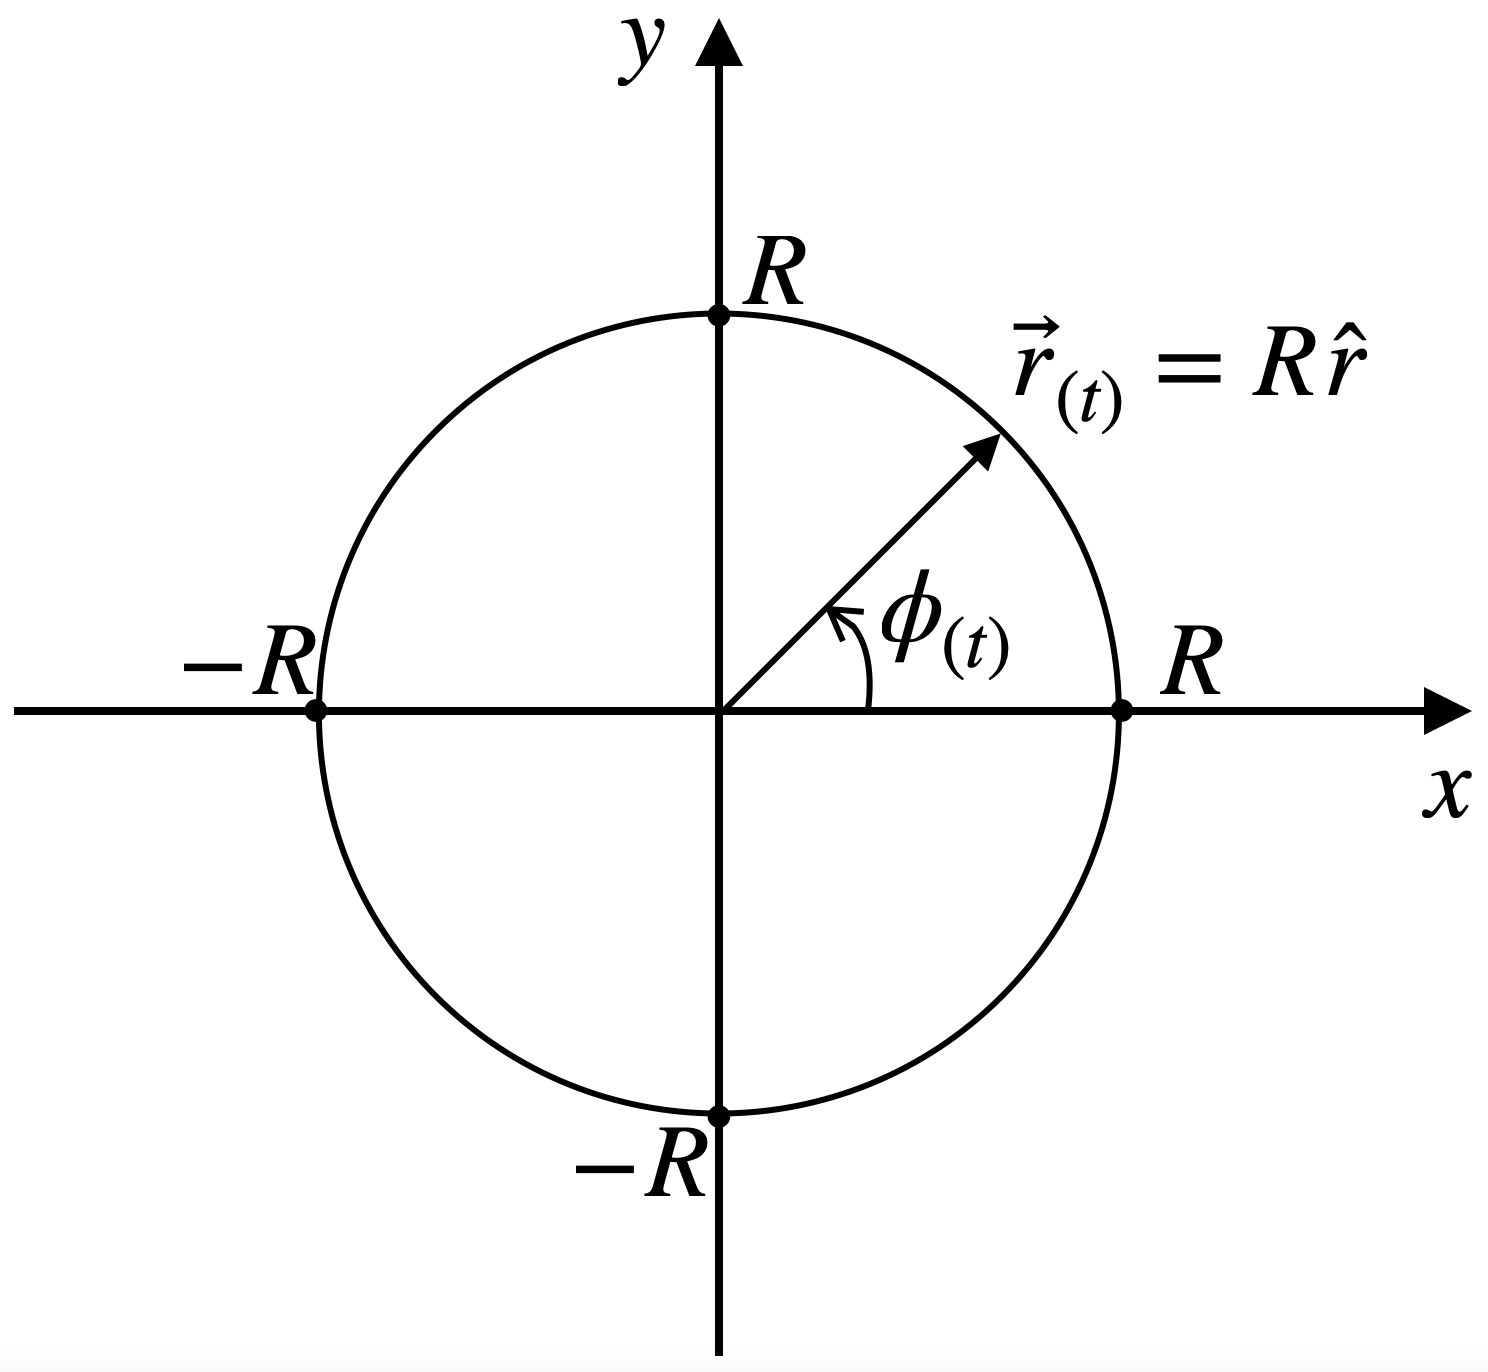
\includegraphics[width=7cm]{images/circ.png}
        \caption{Rappresentazione della traiettoria, del raggio vettore e della variabile angolare $\phi$ nel moto circolare.}
\label{fig:circ}
\end{figure}